\chapter{Testing}
\label{ch:7}

Testing is a critical aspect of software development to ensure the reliability, functionality, and performance of the system. This chapter delves into testing strategies employed in this project. It covers unit testing, integration testing and performance testing to validate the correctness and efficiency of the system.

\section{Unit Testing}

Since this system is going to be available as a public repository that people cannot only use but also modify, it is important for such a project to be well-tested to ensure that key features are still working.

Unit testing focuses on testing individual units or components of the application in isolation to verify that they perform as intended. In the context of this project, unit tests were written to validate the functionality of specific components, functions, or classes within the codebase.

\subsection{Front-End Unit Testing}

One of the features that were noted in section \ref{subsec:processControl} was that the front-end is responsible for managing the state of the system. Therefore, it has several components that must react to system changes. For this reason, unit testing becomes very important to ensure the correctness and reliability of the user interface components and their behaviour. The goal is to validate that the UI components render correctly, respond to user interactions as expected, and maintain their functionality across different scenarios.

\subsubsection{Jest and React Testing Library}

Jest is a JavaScript testing framework. It provides features for writing and executing tests, including assertions and mocking. React Testing Library is a testing utility for React that supports testing components in a way that reminds how they are used by end users.


\subsubsection{Tests}

Given that \texttt{StepInfo} serves as a primary component that the user is going to interact with very frequently, which is also responsible for presenting the process's state, it becomes necessary to test it. 

As it was mentioned in Section \ref{subsec:stepInfo}, the \texttt{StepInfo} component has 4 states, such as \texttt{SelectLocations}, \texttt{DefineAttributes}, \texttt{ScoreAttributes} and \texttt{Result}. In order to maintain the functionality of each stage, I have written the following unit tests:

\begin{itemize}
    \item Test to ensure that \texttt{StepContainer} is rendered correctly when default step\\ \texttt{SelectLocations} is active. It means that the ``Select Locations`` step is highlighted, and the image is displayed when no locations are selected. Also, there is a test to check if it is rendered correctly after the user selects several locations.
    \item Test to ensure that when \texttt{DefineAttributes} step is active, it is rendered correctly, and the user can interact with it.
    \item Test to ensure that when \texttt{DefineAttributes} step is active, and the user fills all the necessary inputs, he is allowed to move to the next step. Additionally, there are several tests for invalid inputs. In this case, the test verifies whether the error message is displayed correctly.
    \item Test to ensure that when \texttt{ScoreAttributes} step is active, it is rendered correctly.
    \item Test to ensure that the final step is rendered correctly.
\end{itemize}

The tests can be found at \texttt{StepInfo.spec.tsx} file. Here is an example of the first test that checks whether components \texttt{StepContainer} and \texttt{StepInfo} were rendered correctly (Listing \ref{lst:jestTest}).

\begin{lstlisting}[caption={Unit test for rendering the StepContainer component.}, label={lst:jestTest}]
it('StepContainer renders correctly', () => {

    // Mock the return value of buildMap
    (buildMap as jest.Mock).mockReturnValue({});

    // Mock the implementation of ImageContent
    (ImageContent as jest.Mock).mockImplementation(() => <>Image</>);

    // Render the component under test
    render(
      <StepsContainer>
        <StepInfo />
      </StepsContainer>
    );

    // Assert that the mocked component is rendered correctly
    expect(screen.getByTestId(StepInfoTest.stepContainer)).toBeInTheDocument();

    // Assert if SelectLocations step is active by default
    expect(screen.getByTestId(icons.location)).toHaveClass("current");

    // Assert if default image is displayed
    expect(screen.getByText(/image/i)).toBeInTheDocument();
});
\end{lstlisting}

\subsection{Back-End Unit Testing}

Back-end testing for this system is crucial to ensure that the server-side logic functions correctly and handles requests appropriately with different inputs. The back-end is highly configurable; it is a core of the system. It sets up front-end application based on datasets and configuration provided by the user. Therefore, it is necessary to ensure that the system works correctly in case of any errors or unexpected inputs.

\subsubsection{Pytest}

Pytest is a popular testing framework for Python that offers a simple syntax and powerful features for writing and executing tests. It provides capabilities for assertions, fixtures, parameterized testing, and mocking, making it well-suited for testing web applications built with frameworks like FastAPI.

\subsubsection{Tests}

To validate the server's functionality, there are several tests to ensure the proper operation of each endpoint. The testing involves simulating a user request and afterwards comparing its output with the expected result. While this process is straightforward for \texttt{GET} requests, I have implemented additional tests for \texttt{POST} requests with invalid data. This ensures that the server appropriately handles such scenarios.

It is important to mention that I have also created a specific configuration file \texttt{init.yaml}, containing generated datasets. This configuration file serves the purpose of generating consistent outputs, which allowed me to compare them with the expected results during testing. Configuration files and datasets for testing can be found in \texttt{/server/tests} folder. Additionally, I have added tests to check that the configuration file is processed correctly and that \texttt{get\_geocompetition} caches results.

The tests can be found in \texttt{/server/test.py} file. Here is an example of a unit test for processing configuration file \texttt{init.yaml} (Listing \ref{lst:pytest}). 

\begin{lstlisting}[caption={Unit test for retrieving configuration settings.}, label={lst:pytest}]
def test_get_config(monkeypatch):
    monkeypatch.setenv("TESTING", "True")
    
    datasets = config.competitors.keys()

    expect = {
        "center": get_coordinates(config.area),
        "datasets": list(datasets),
        "grid": get_squares_list()
    }

    response = client.get(Urls.Config.value)
    assert response.status_code == 200
    assert response.json() == json.loads(json.dumps(expect))
\end{lstlisting}

\section{Performance Testing}
\label{sec:performanceTesting}

In the context of this project, performance testing is essential due to the complexity of the \texttt{get\_geocompetition} function that calculates areas with high competition for the provided dataset. The time taken for these calculations can vary significantly based on the size of the datasets provided because of the algorithm's time complexity $O(n^2)$.

\subsection{Planning and Preparation}

In order to measure execution time, \texttt{time}\footnote{Time library---\url{https://docs.python.org/3/library/time.html}} library was used.\\At the beginning of \texttt{get\_geocompetition} function, the \texttt{time} method was called for the first time, and its result was assigned to \texttt{start\_of\_execution}, at the very end of the same function method \texttt{time} was called again and, its result was assigned to \texttt{end\_of\_execution}. Subtracting \texttt{start\_of\_execution} from \texttt{end\_of\_execution} allowed me to determine the execution time.

\subsection{Testing Process}

The following steps outline the testing process:

\begin{itemize}
    \item Generate different datasets with varying sizes and characteristics to represent realistic scenarios. All the generated datasets that were used in this testing can be found in the folder \texttt{/server/tests/performance}.
    \item Run the application with each dataset and measure the time taken to perform the calculations. Repeat the tests multiple times to ensure consistency and accuracy of results.
    \item Analyze the performance test results to identify trends (Table \ref{tab:performance}).
\end{itemize}

\subsection{Results}

Table \ref{tab:performance} presents the time required to calculate datasets of varying sizes, ranging from $10\times10$ to $1000\times1000$ entries (Number of potential customers $\times$ number of competitors). 

The dataset size represents the dimensions of the dataset, while the "Entries" column indicates the total number of data points within each dataset. The "Time (seconds)" column specifies the duration taken by the application to process and analyze the datasets.

\begin{table}[ht]
\centering
\begin{tabular}{|c|c|c|}
\hline
\textbf{Dataset Size} & \textbf{Entries} & \textbf{Time} \\ \hline
\multirow{1}{*}{$10\times10$} & 100 & 1.7 seconds \\ \hline
\multirow{1}{*}{$100\times100$} & 10,000 & 35.38 seconds \\ \hline
\multirow{1}{*}{$1000\times1000$} & 1,000,000 & 908.37 seconds \\ \hline
\end{tabular}
\caption{Time taken to calculate datasets of varying sizes}
\label{tab:performance}
\end{table}

\subsection{Conclusion}

In conclusion, the performance testing conducted on the \texttt{get\_geocompetition} function has provided valuable insights into its efficiency and scalability. The function's execution time was observed to be influenced significantly by the size of the datasets processed, owing to its time complexity of $O(n^2)$. It is important to note that the function implements several caching and optimization techniques, detailed in Section \ref{subsec:gridBasedOptimization}, which impact its overall performance.

\section{Testing Application with Real Data}
\label{sec:testingApplicationWithRealData}

Testing the application with real data is essential to validate its functionality and performance under realistic conditions. This particular test will be used in order to show the potential users and contributors how the system functions.

These are the steps to run and utilize this application effectively:

\begin{itemize}
    \item Configure the back-end by creating and modifying the \texttt{init.yaml} file.
    \item Enable the application to assess newly incorporated datasets.
    \item Begin utilizing the application.
\end{itemize}

\subsection{Configuration}

In configuration, we must specify three crucial elements: geographic area, the dataset containing potential customers, and the datasets of competitors. It's essential that all datasets originate from the same geographic area.

In the context of geographical location, I will use "Brno, Czech Republic." As discussed in section \ref{subsec:dataRequirements}, the datasets suitable for meeting the system's data needs include "Number of people living at addresses" and "Brno retail research". I have acquired both datasets. However, upon review of section \ref{subsec:dataRequirements}, it's evident that both datasets differ significantly from the specified data format outlined in section \ref{section:datasetFormat}. Therefore, it is necessary to parse both datasets to align them with the required format.

\subsubsection{Parsing Dataset with Customers}
Dataset with customers refers to a dataset with a number of people living at addresses. Using a Python script, the dataset was transformed into a format compatible with the application (Listing \ref{lst:parsedCustomerDataset}).

\begin{lstlisting}[caption={Result of a parsed dataset},label={lst:parsedCustomerDataset}]
[
    [49.17789499100007, 16.581255326000075, 4], 
    [49.164724902000046, 16.578846962000057, 5], 
    ...,
    [49.16660763800007, 16.583760249000022, 49]
]
\end{lstlisting}

Here is an example of a Python script that was used (Listing \ref{lst:parserCustomerDataset}).

\begin{lstlisting}[caption={Parser written in python to parse the dataset.},label={lst:parserCustomerDataset}]
def serialize_customers():
    customers = read_json_file(CUSTOMERS, Customers)
    
    features = []
    for feature in customers.get("features"):
        count = feature.get("properties").get("pocet")
        lng = feature.get("geometry").get("coordinates")[0]
        lat = feature.get("geometry").get("coordinates")[1]
        features.append((lat, lng, count))
        
    write_json_file("customers-formatted.json", features)
\end{lstlisting}

\subsubsection{Parsing Datasets with Competitors}

The dataset with competitors refers to the dataset of ``Brno retail research``. It was parsed the same way as the dataset with a number of people, using Python script. 

Additionally, it was divided into multiple datasets based on business category \texttt{sluzba\_typ}, such as grocery stores, pharmacies, or restaurants.

\subsection{Data Evaluation}

Data evaluation involves the system automatically assessing the provided data to pinpoint regions characterized by highly competitive areas, indicating a relatively high trading area. This process activates upon the user launching the back-end application, and its results will be then cached for future reuse. For Brno, the evaluation of all the provided datasets in total utilized $84$ threads and took a total of $1971.31$ seconds. It's worth mentioning that the results may differ depending on the number of threads available on the system where the evaluation was initiated.

\subsection{System Launch}

Once the evaluation is done, the user can launch the front-end application to start working with the system (Figure \ref{fig:workingApplication}).

\begin{figure}[ht]\centering
  \centering
  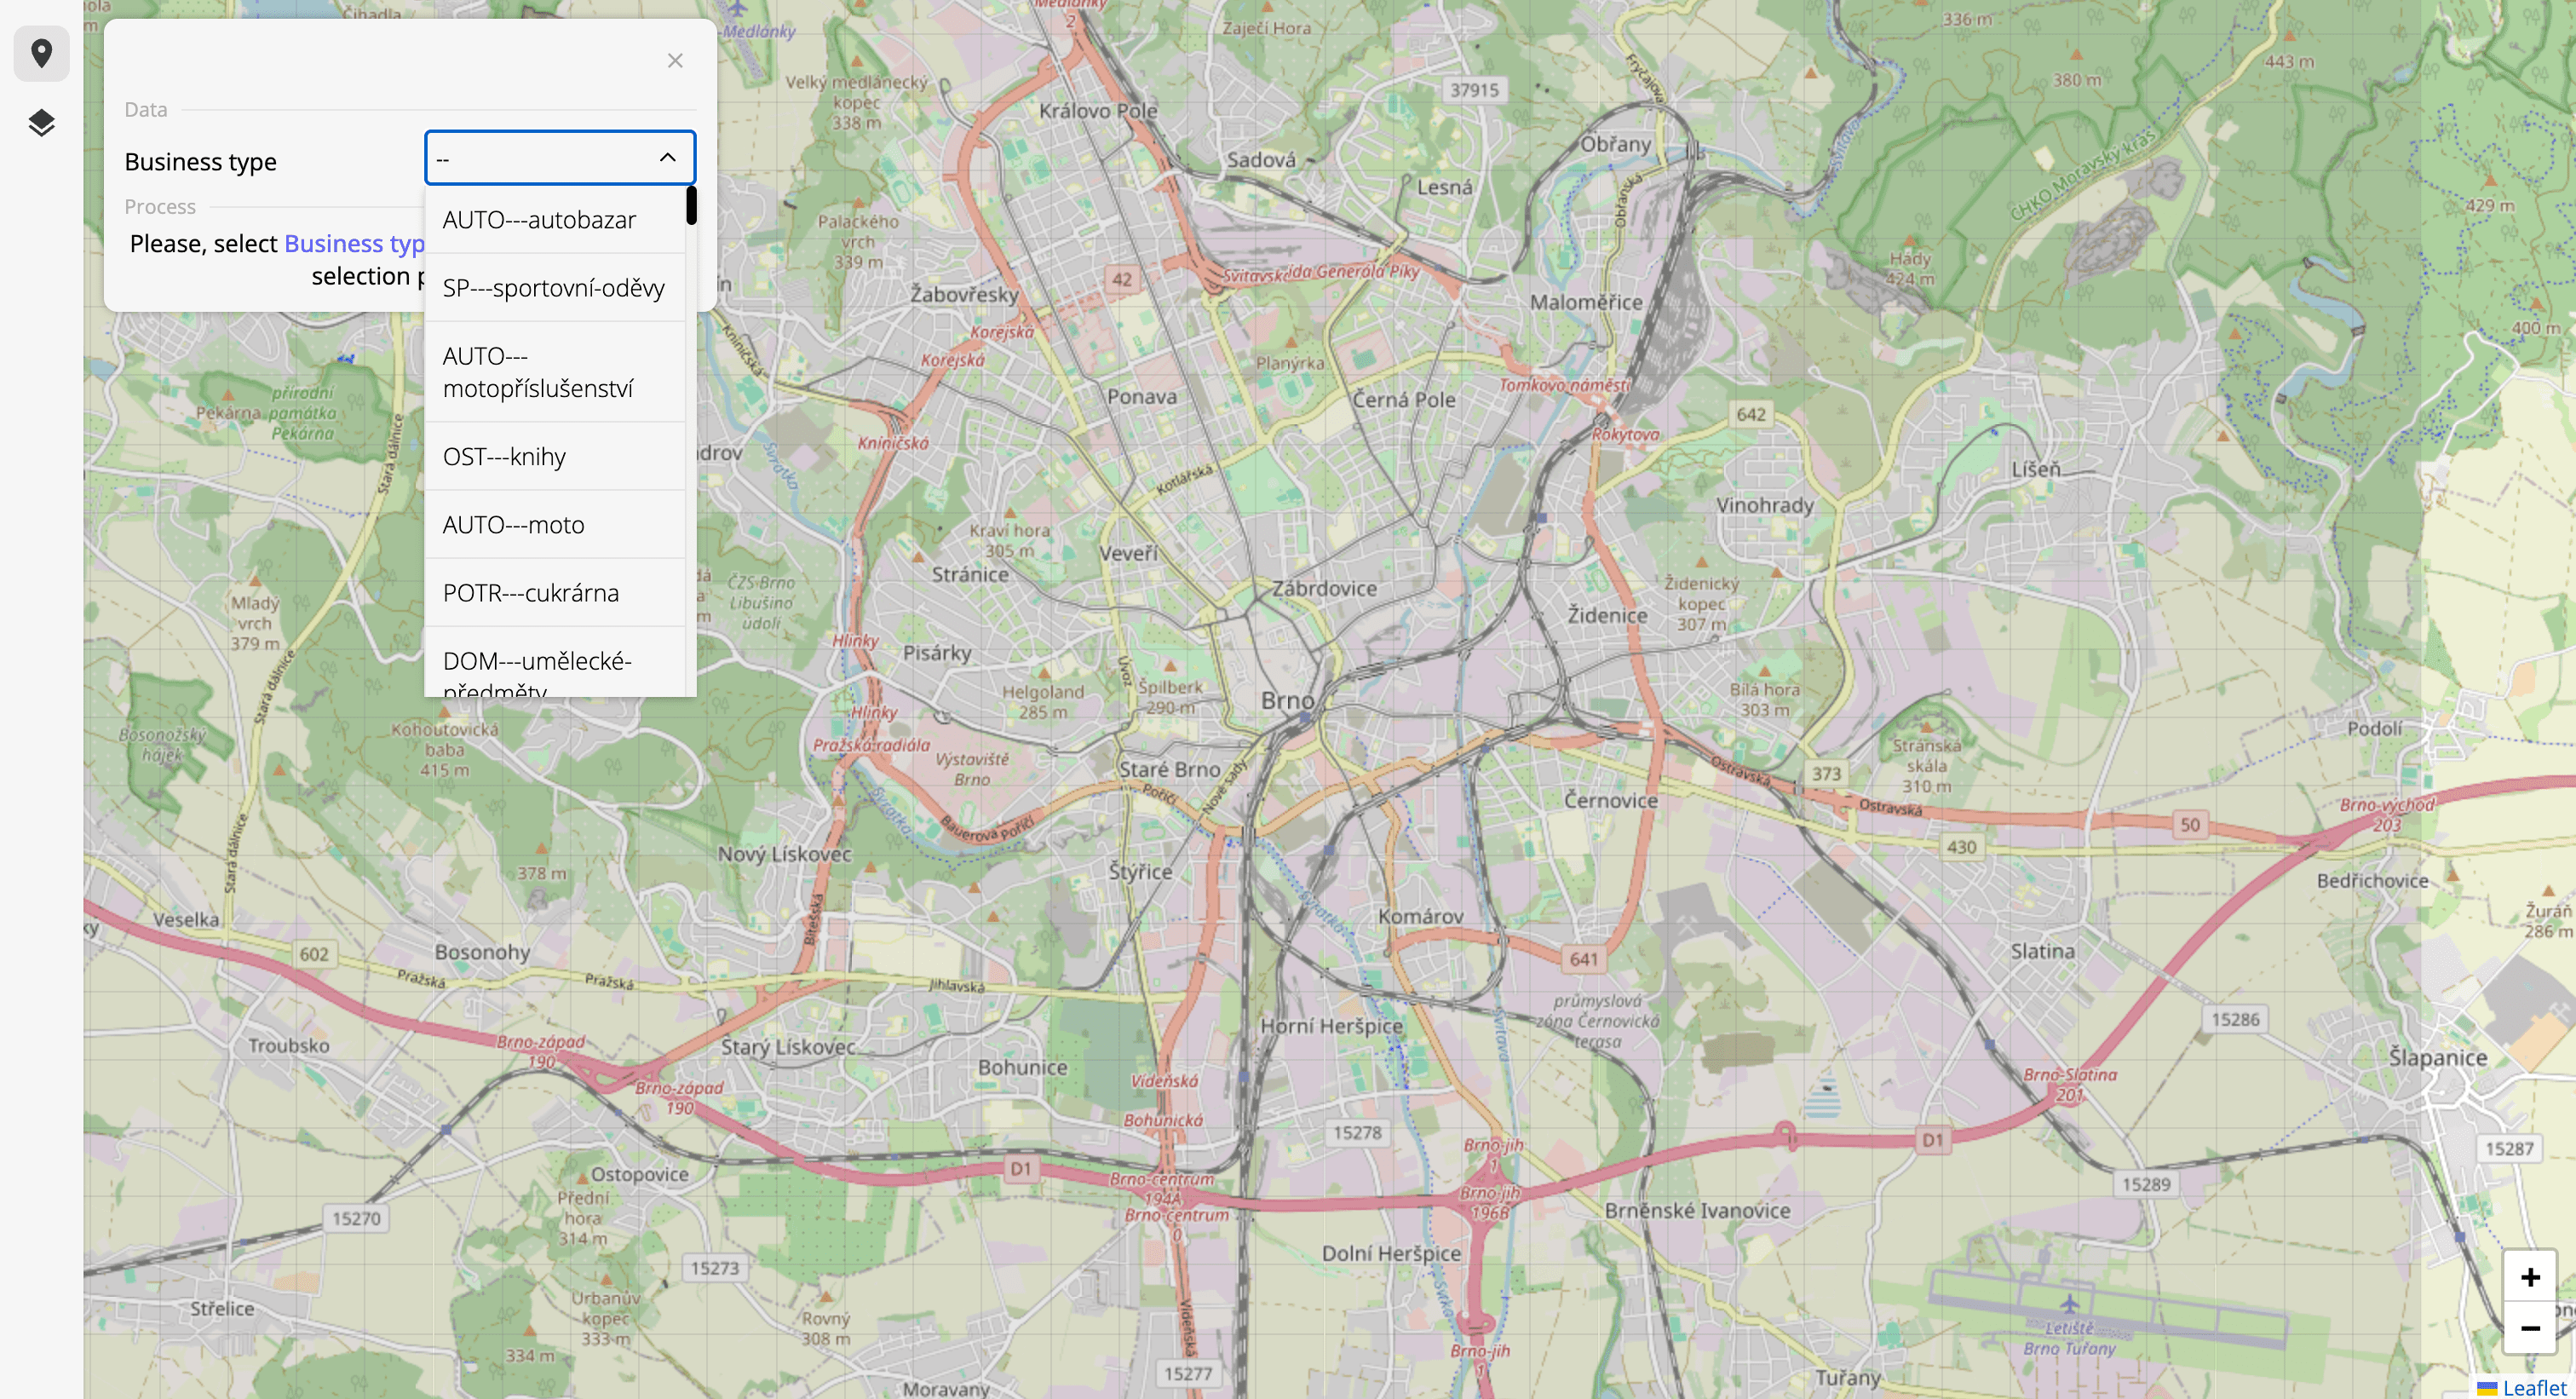
\includegraphics[width=1\linewidth]{obrazky-figures/ch7/system-launch.png}
  \caption{Screenshot of a working application.}
  \label{fig:workingApplication}
\end{figure}

\section{User Testing}

As outlined in section \ref{section:target-audience}, the target audience for this system includes individuals lacking technical proficiency in retail analysis. Therefore, it is crucial to demonstrate the system to these individuals to gather feedback and drive further enhancements.

\subsection{Objective}

The testing scenario aims to confirm that users can successfully navigate the entire decision-making process facilitated by the system and obtain the desired results.

\subsection{Participants}

Three student participants, aged 19-23, took part in the study, with no level of expertise in retail analysis. Each participant was introduced to the system and provided with the following objective: ``Imagine yourself as someone wanting to open a store, restaurant, or cafe and facing challenges in selecting the optimal location. Use this application to fulfil this objective.``

\subsection{Testing Environment}

As all participants were from Brno, the system was configured with data specific to this location to ensure participants felt familiar with the area. 

\subsection{Gathered Feedback}
\label{section:feedback}

During the testing sessions, participants often encountered difficulties in understanding the steps of the process or understanding the displayed information. For instance:

\begin{itemize}
    \item During the site selection stage, two participants were uncertain about the purpose of the heatmap feature and what it represents in the application, and one participant did not realize that locations needed to be selected in this step.
    \item When defining attributes for the sites, one participant expressed confusion about the types of attributes that could be specified.
    \item Participants pointed out that the project lacks an introduction, a description of specific UI components detailing their functions and how to interact with them, as well as an explanation of the utilized data.
\end{itemize}


\subsection{Improvements}

In response to the feedback collected in section \ref{section:feedback}, the following enhancements have been implemented in the front-end application:

\begin{itemize}
    \item Each step now includes a brief description outlining the information presented to the user and the actions required at that particular stage. These descriptions have been incorporated into modal window components and the \texttt{StepInfo} component (Figure \ref{fig:improvementHints}).

    \item When defining attributes, the user will be provided with suggested attributes and an explanation of what could be specified as a value (Figure \ref{fig:improvementDefineAttributes}).

    \item I have developed a separate page containing an introduction to the project, its UI components, and the utilized data. Users can also access a demo video demonstrating the entire site selection process (Figure \ref{fig:tutorial}).
\end{itemize}

\begin{figure}[ht]\centering
  \centering
  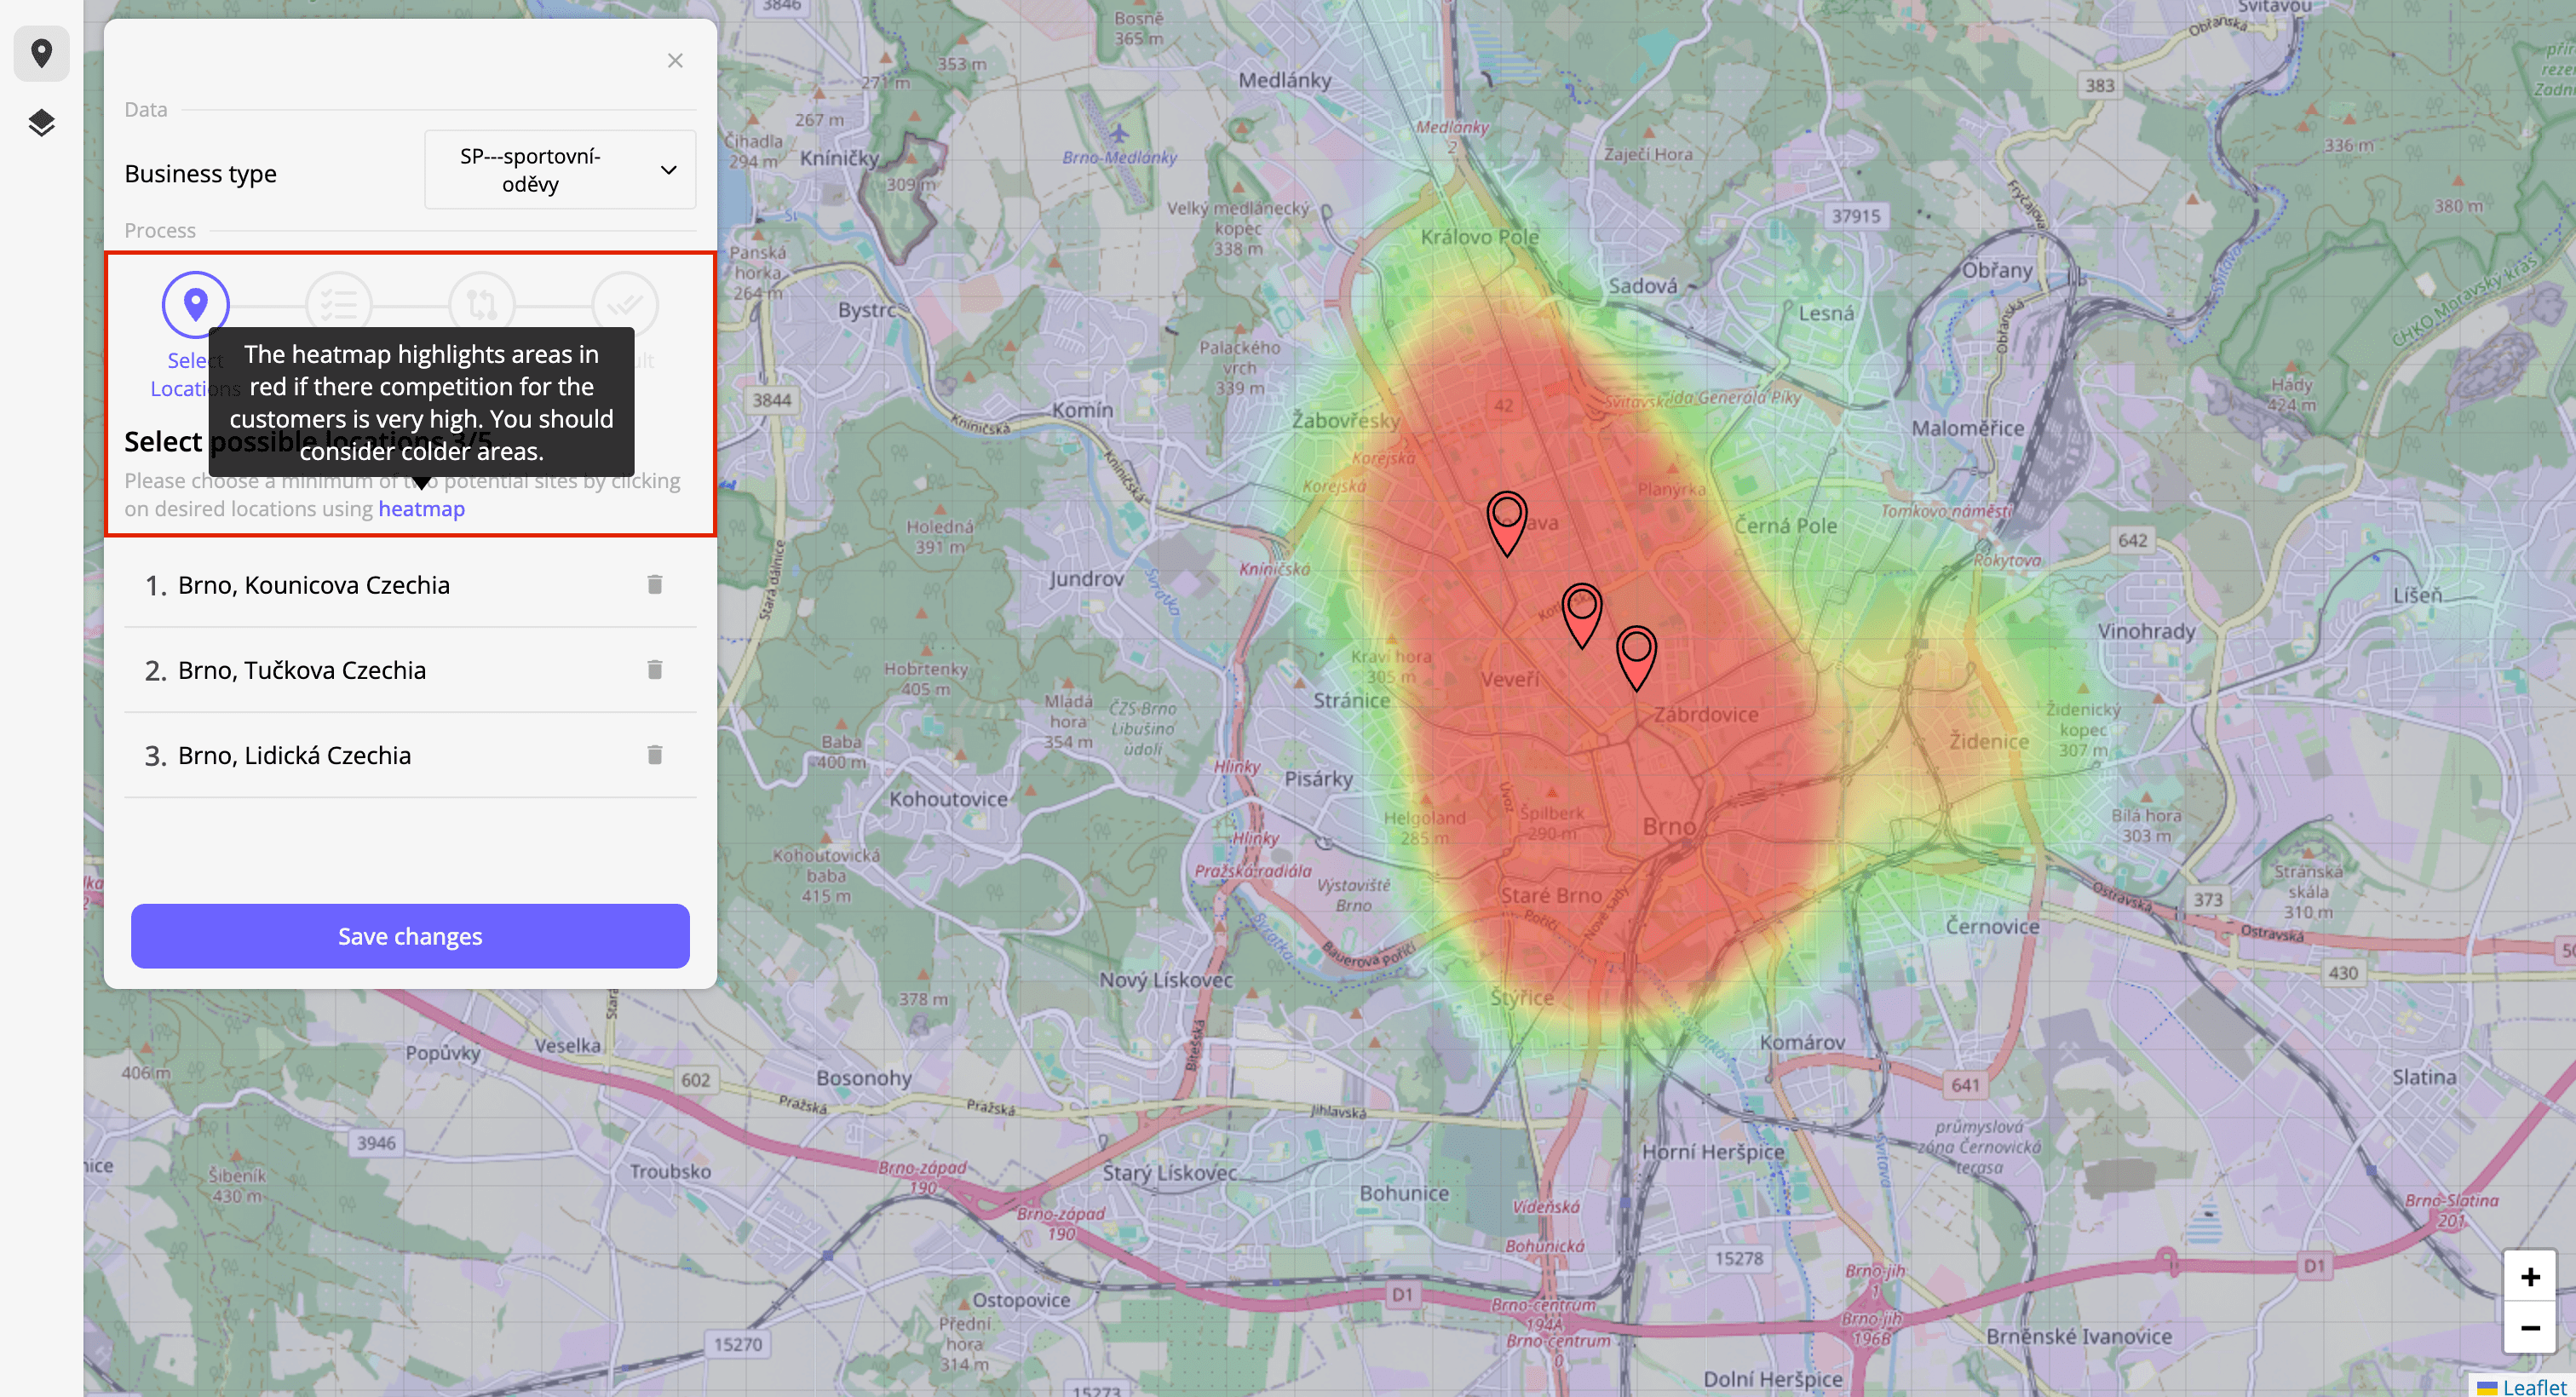
\includegraphics[width=0.9\linewidth]{obrazky-figures/ch7/improvement-hints.png}
  \caption{Hints and tooltips for the user to navigate.}
  \label{fig:improvementHints}
\end{figure}

\begin{figure}[ht]\centering
  \centering
  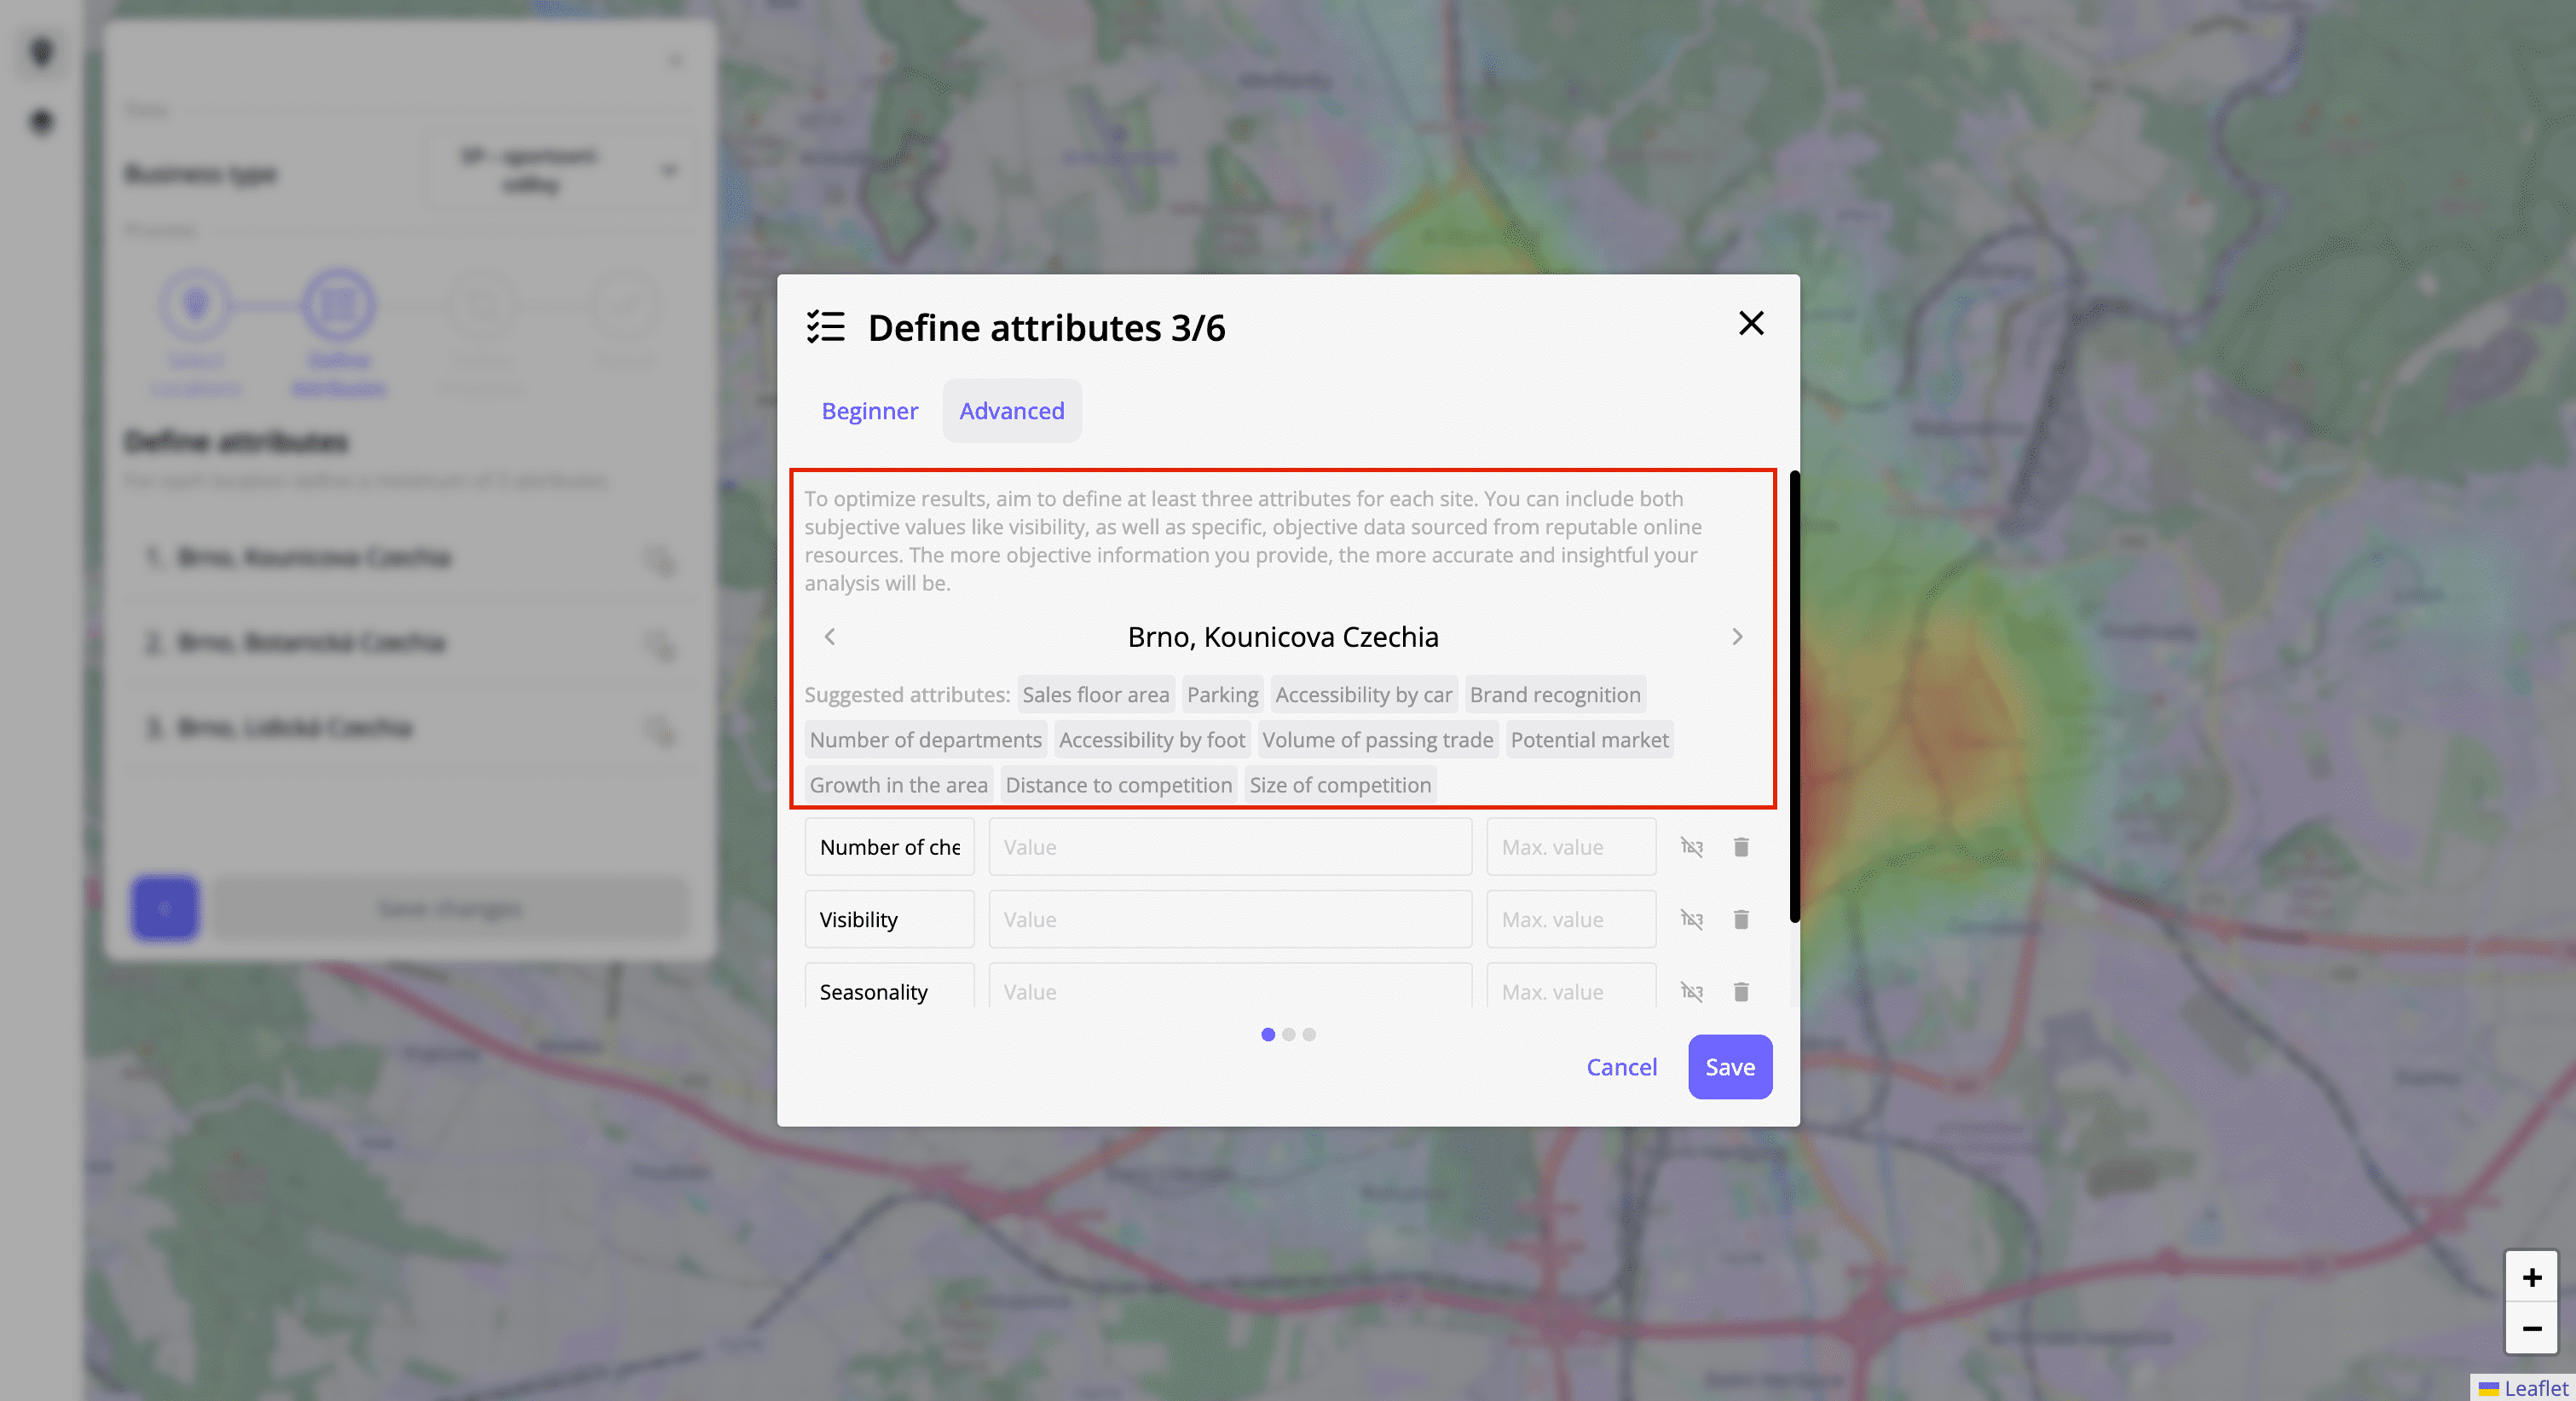
\includegraphics[width=0.9\linewidth]{obrazky-figures/ch7/improvement-define-attributes.png}
  \caption{Suggested attributes and help for the user when defining attributes.}
  \label{fig:improvementDefineAttributes}
\end{figure}

\begin{figure}[ht]
  \centering
  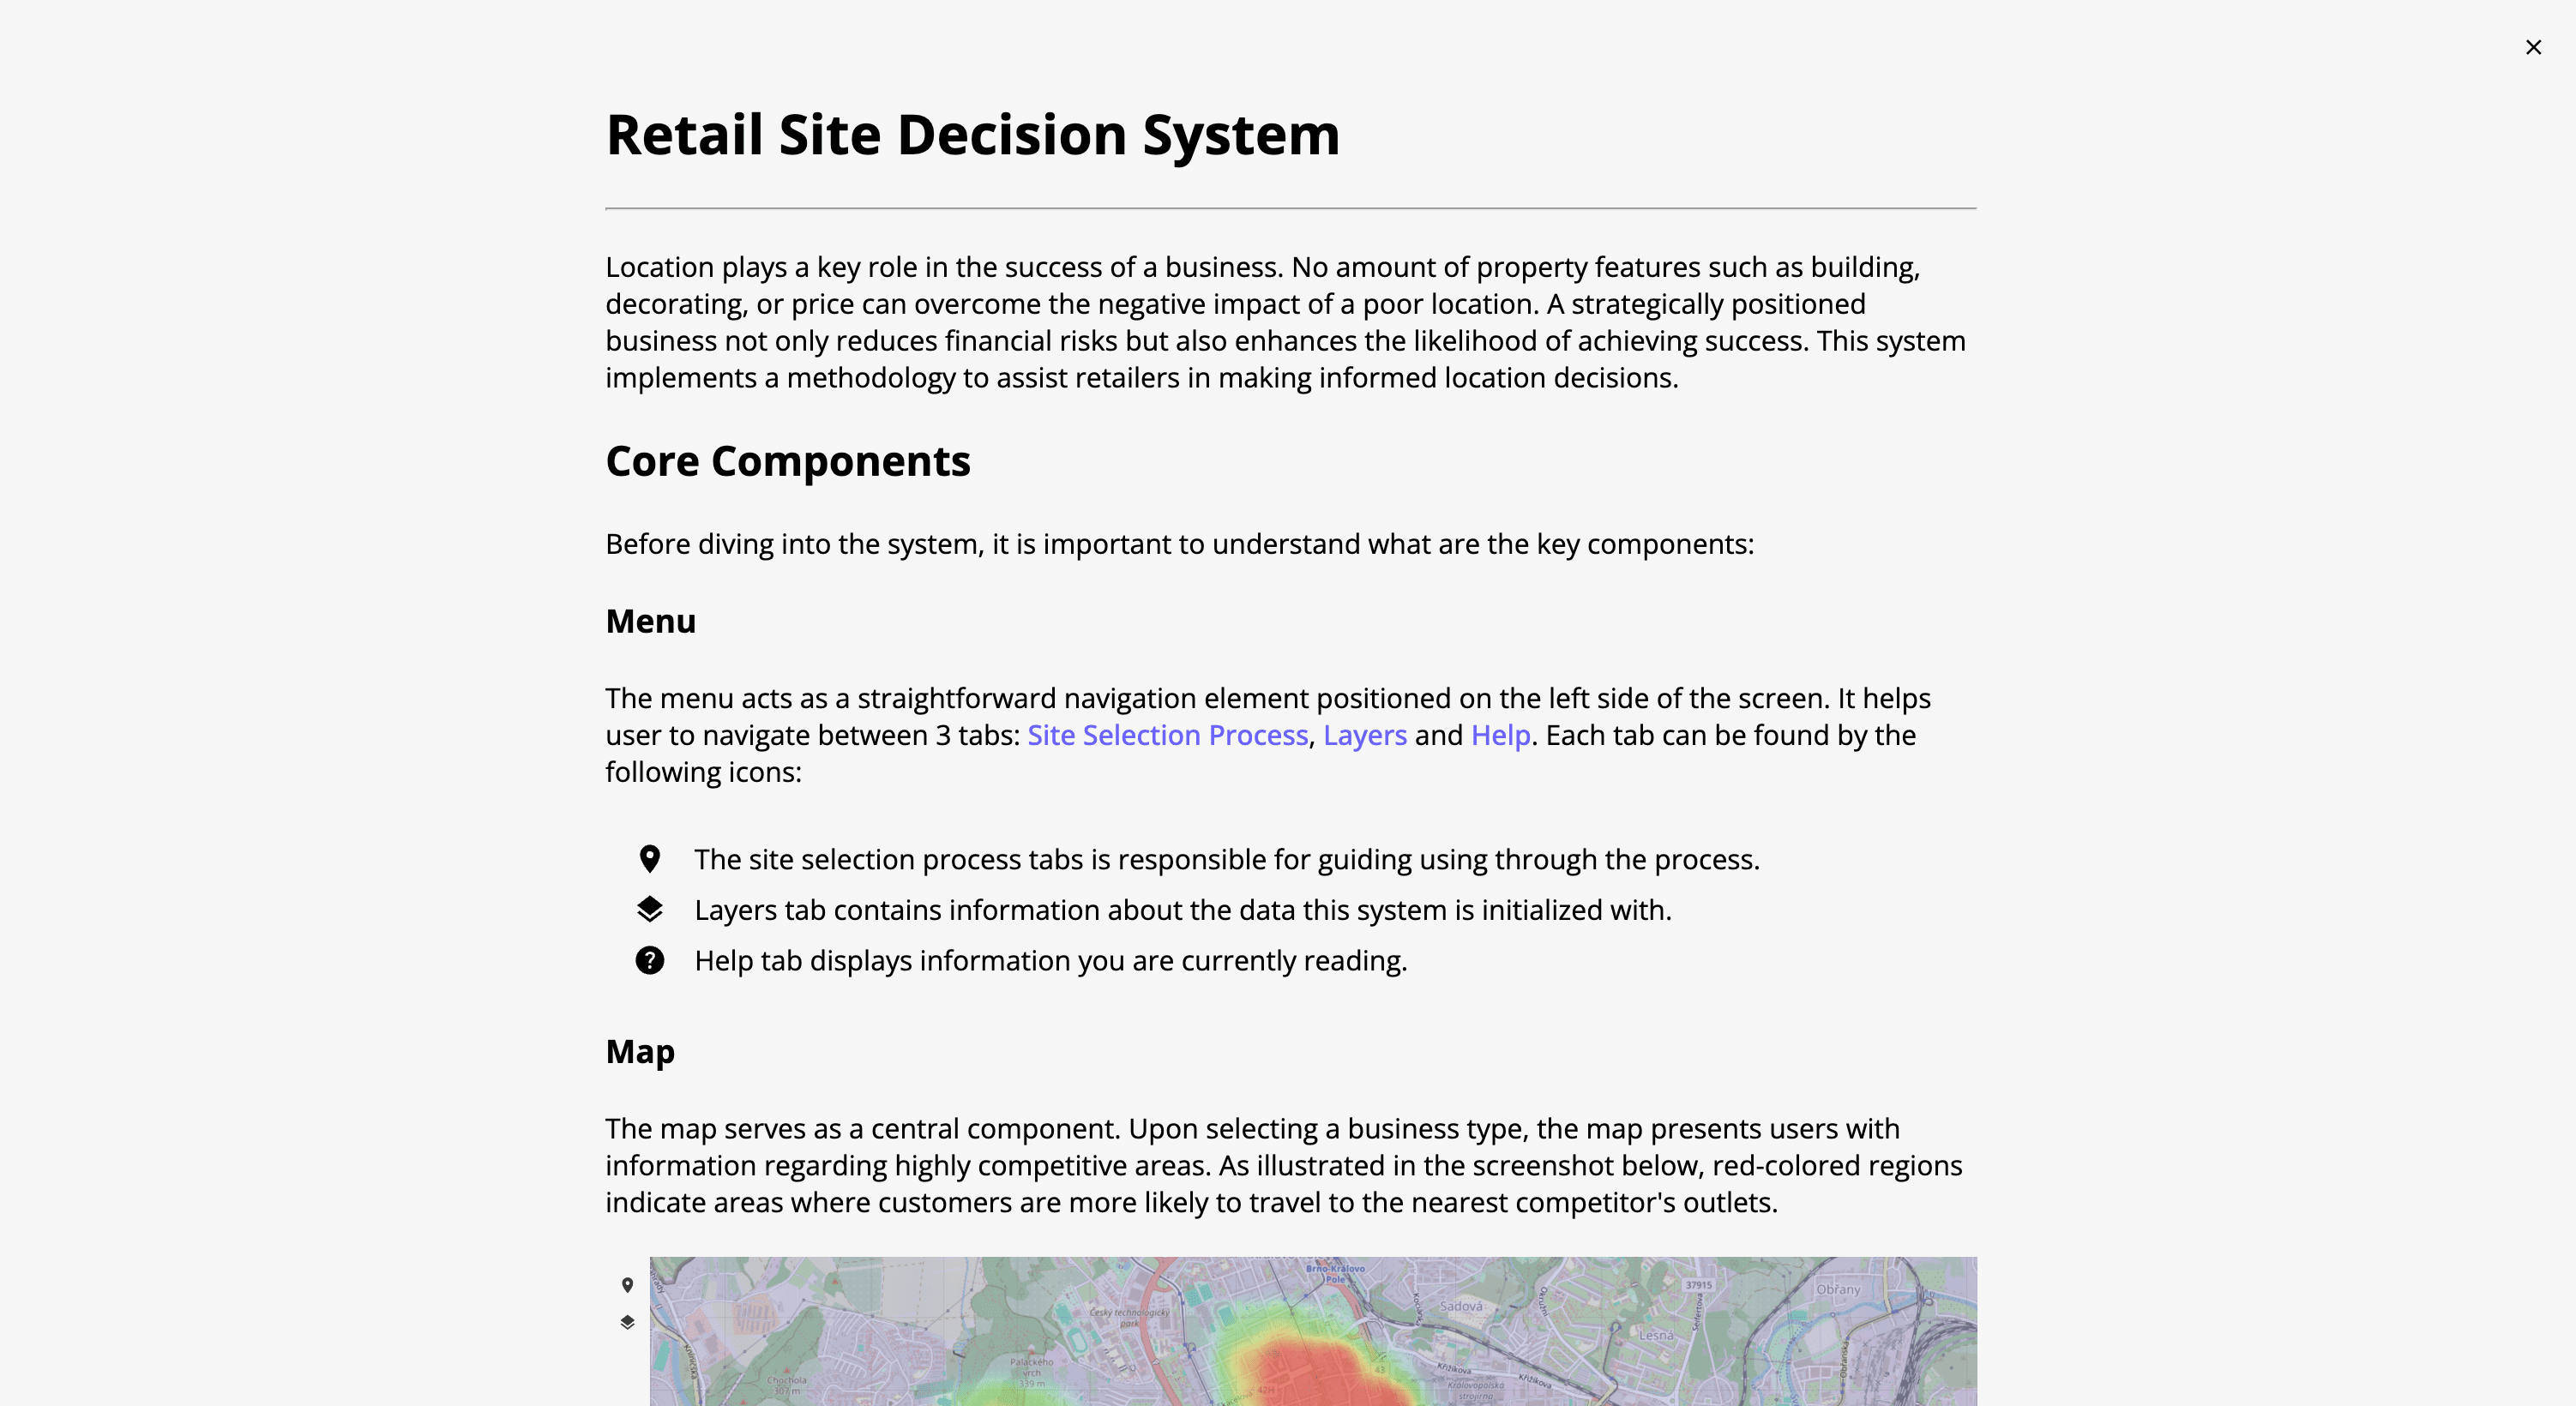
\includegraphics[width=1\linewidth]{obrazky-figures/ch7/tutor1.png}
  \vspace{10pt}
  \vspace{10pt}
  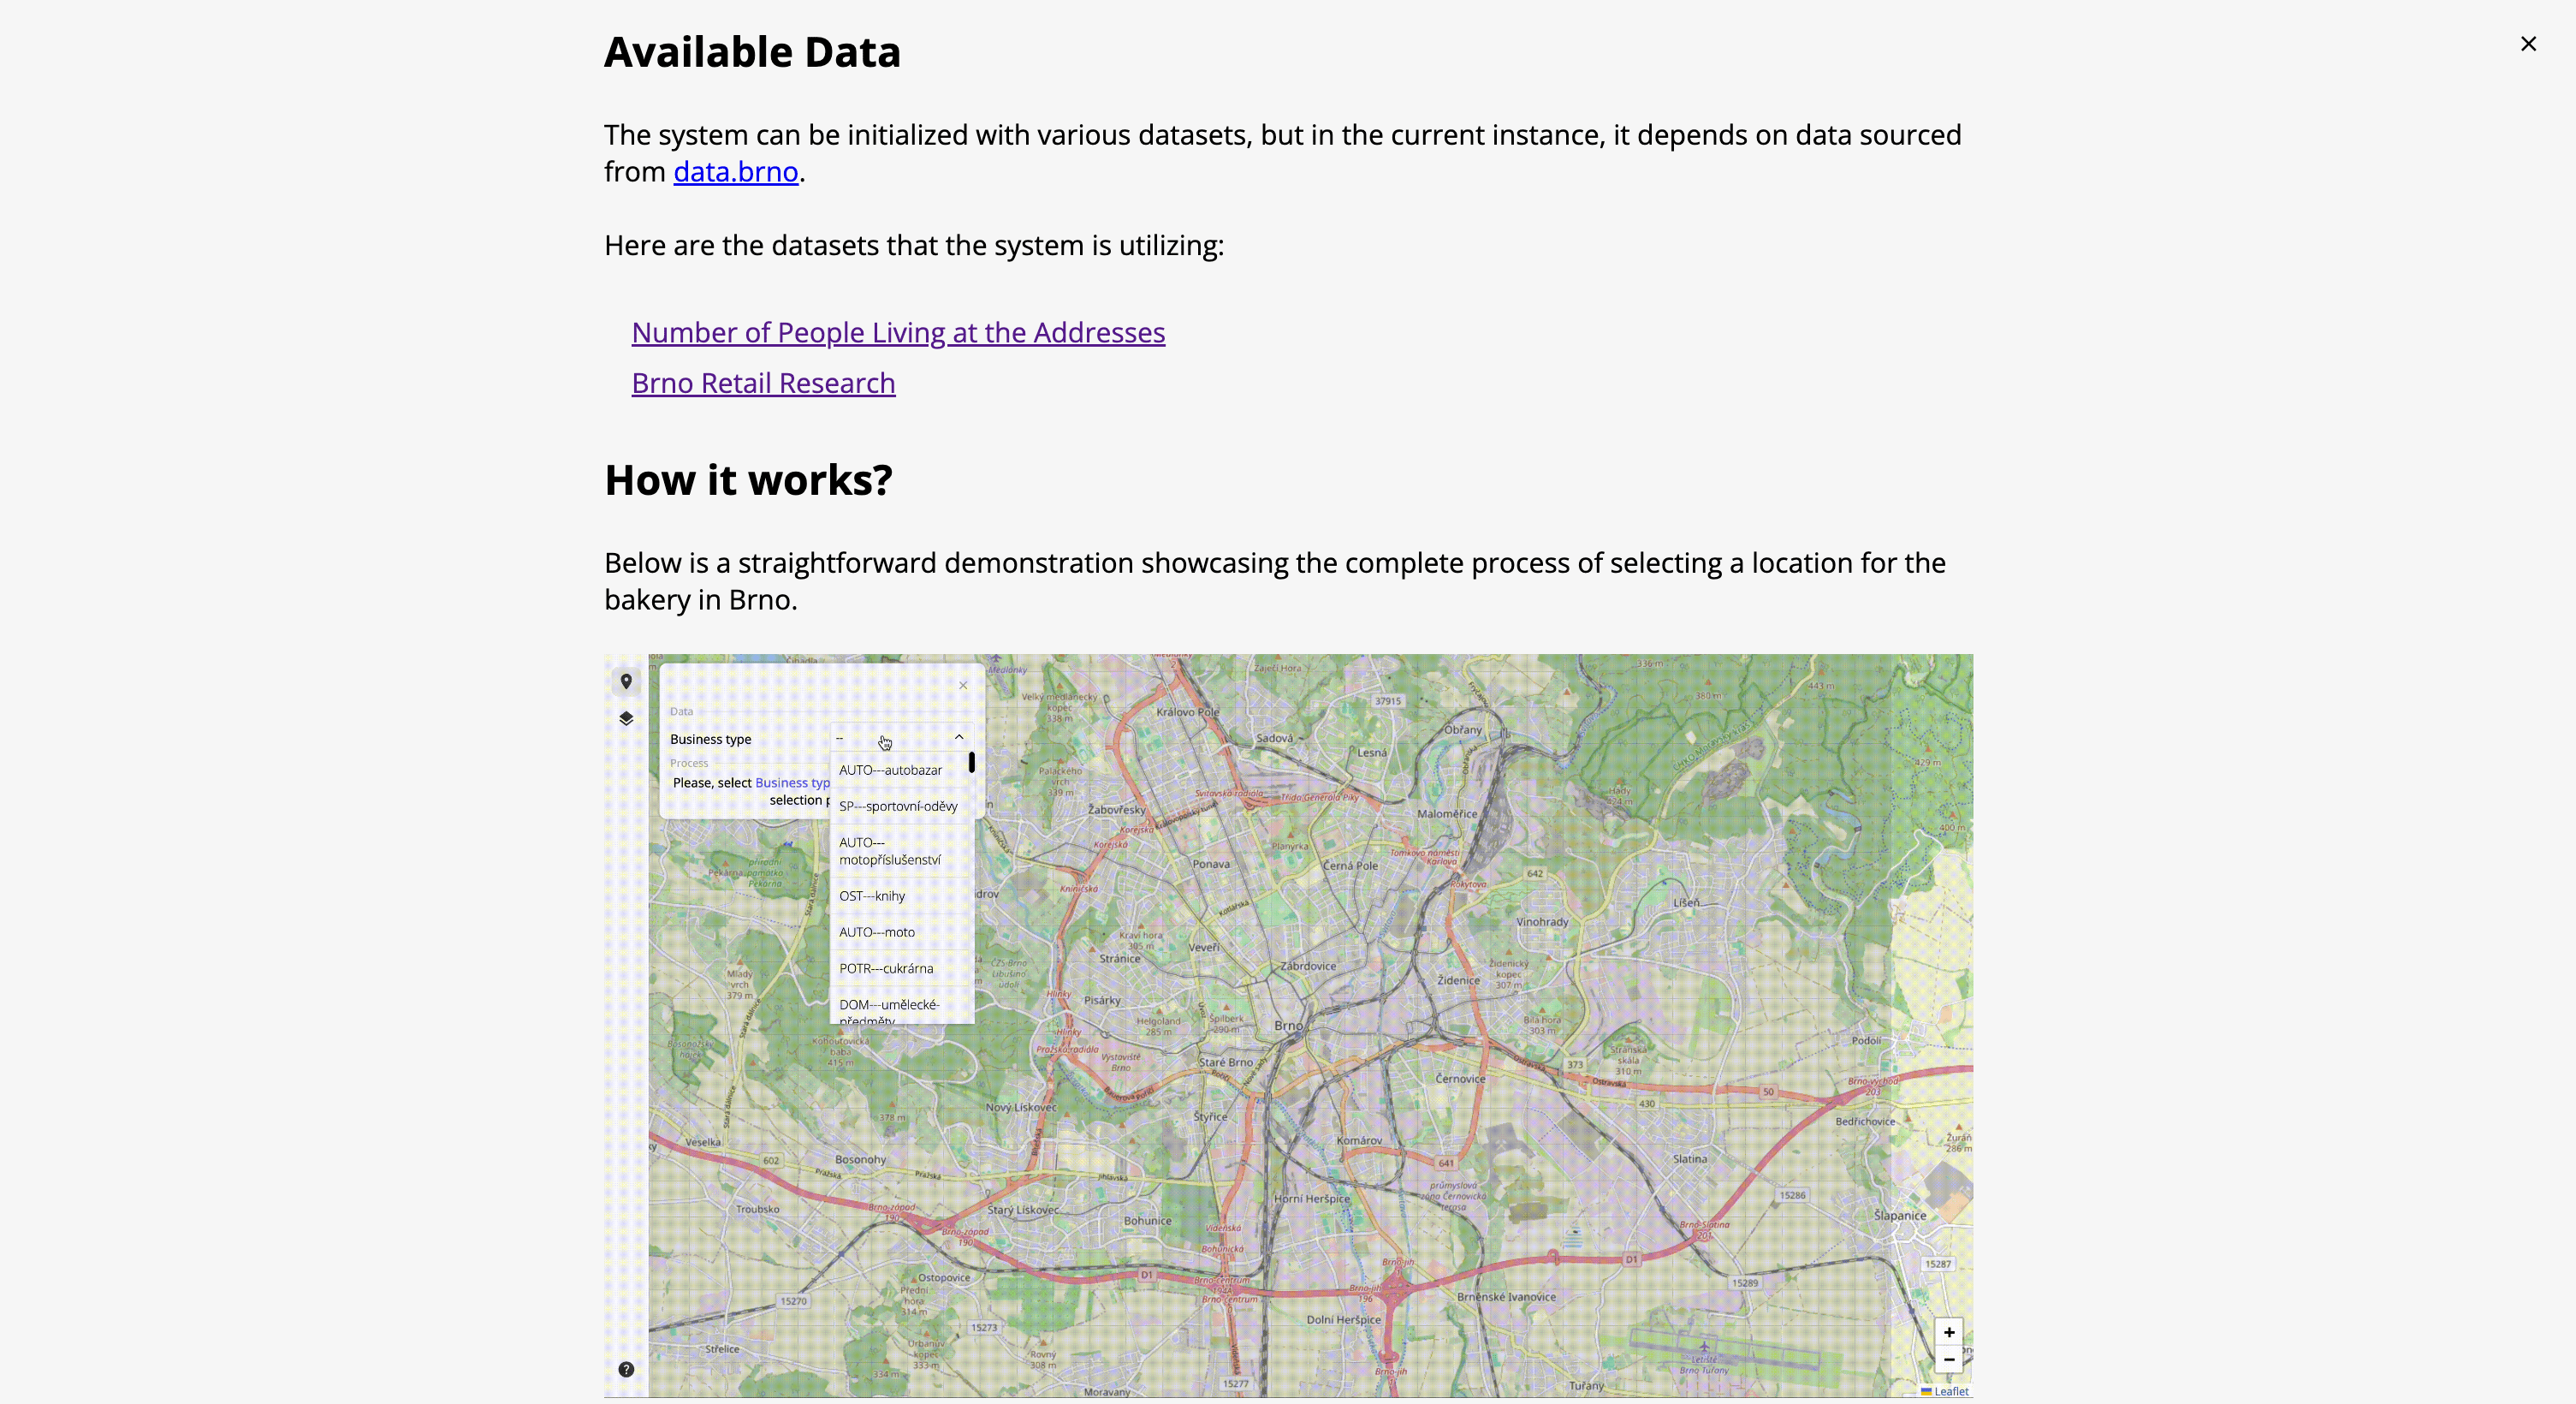
\includegraphics[width=1\linewidth]{obrazky-figures/ch7/tutor2.png}
  \caption{Page with introduction to the project and tutorial to use it.}
  \label{fig:tutorial}
\end{figure}
